\chapter{Time Will Tell: The role of mobile learning analytics in self-regulation} 


\vfill
Nowadays, smartphone users bla bla
\vspace{3em}

This chapter has been submitted as: 
Tabuenca, B., Kalz, M., \& Specht, M. (2015). (Submitted) Time Will Tell: The role of mobile learning analytics in self-regulation. \em Internet and Higher Education \em

\clearpage

\section{Introduction}

\subsection{Self-regulation with mobile technology}

\subsubsection{Psychology of notifications}

\subsubsection{Learning analytics}

\subsubsection{Seamless learning}

\section{Method}

\subsection{Participants}

\subsection{Materials}

\subsubsection{LearnTracker Backend}


\begin{figure}
     \centering
     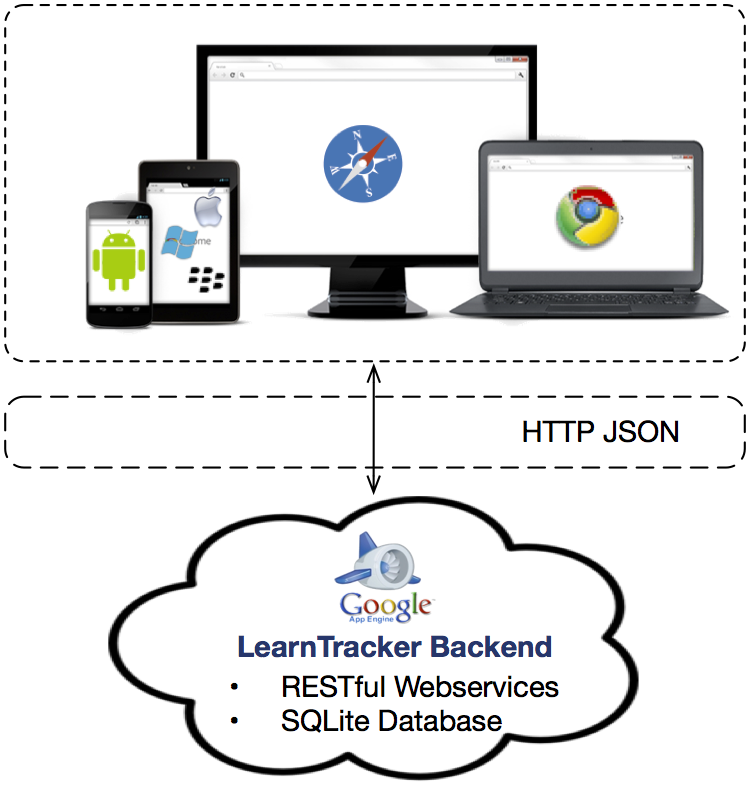
\includegraphics[width=0.7\linewidth]{img/studyload_fig1}
     \caption{LearnTracker's Backend outline}
     \label{fig:sload_1}
\end{figure}
\textbf{Database model}


\begin{figure}
     \centering
     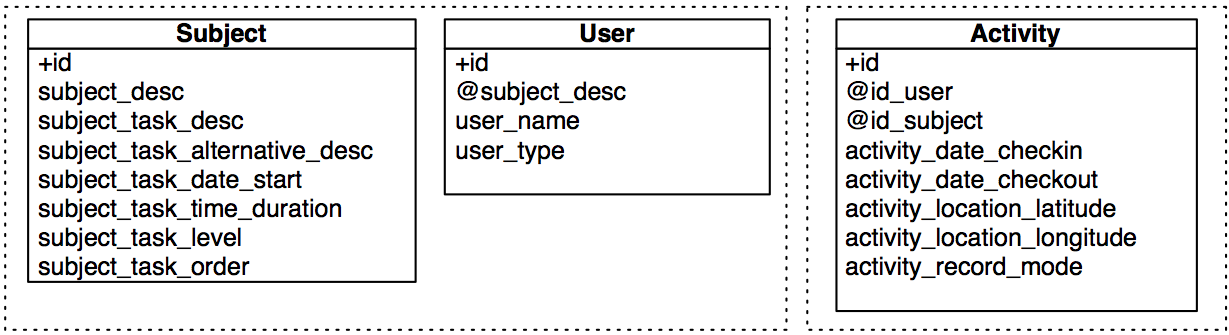
\includegraphics[width=0.7\linewidth]{img/studyload_fig2}
     \caption{LearnTracker's Backend database model}
     \label{fig:sload_2}
\end{figure}

\textbf{Webservices}


\subsubsection{Mobile clients}

\textbf{LearnTracker for Android}

\begin{center}
\begin{figure}[ht]
\centering
	\subfloat[Yardstick comprising activities scheduled in the GIS course]{
		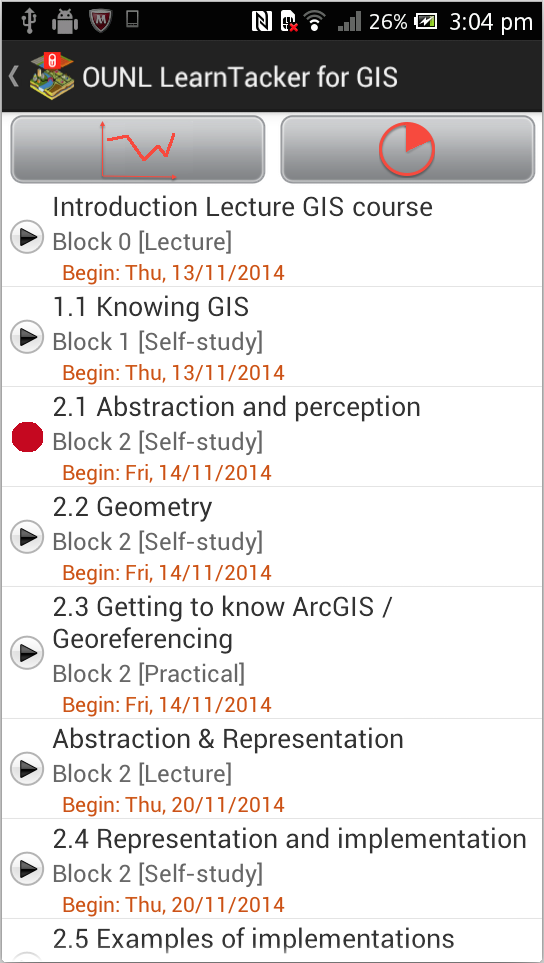
\includegraphics[width=0.3\linewidth]{img/studyload_fig3a}
		\label{fig:sload_3a}
	}
	\subfloat[Check-in: Tap to start learning activity ''2.1 Abstraction and perception'']{
		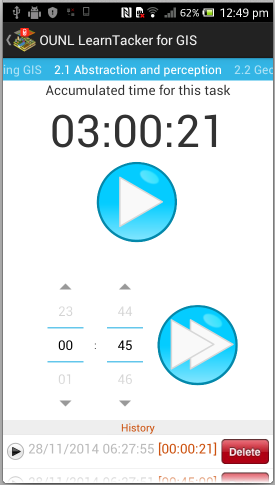
\includegraphics[width=0.3\linewidth]{img/studyload_fig3b}
		\label{fig:sload_3b}
	}	
	\subfloat[Check-out: Tap to stop learning activity  ''2.1 Abstraction and perception'']{
		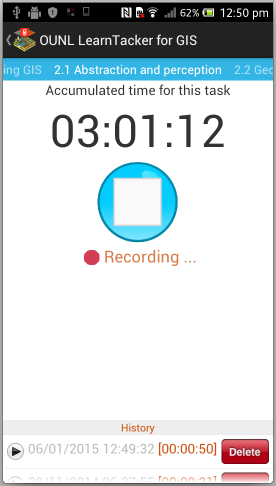
\includegraphics[width=0.3\linewidth]{img/studyload_fig3c}
		\label{fig:sload_3c}
	}	
      \caption{LearnTracker client for Android}
      \label{fig:sload_3}
\end{figure}
\end{center}

\begin{center}
\begin{figure}[ht]
\centering
	\subfloat[PieChart. Time devoted by a student on the activities in a course]{
		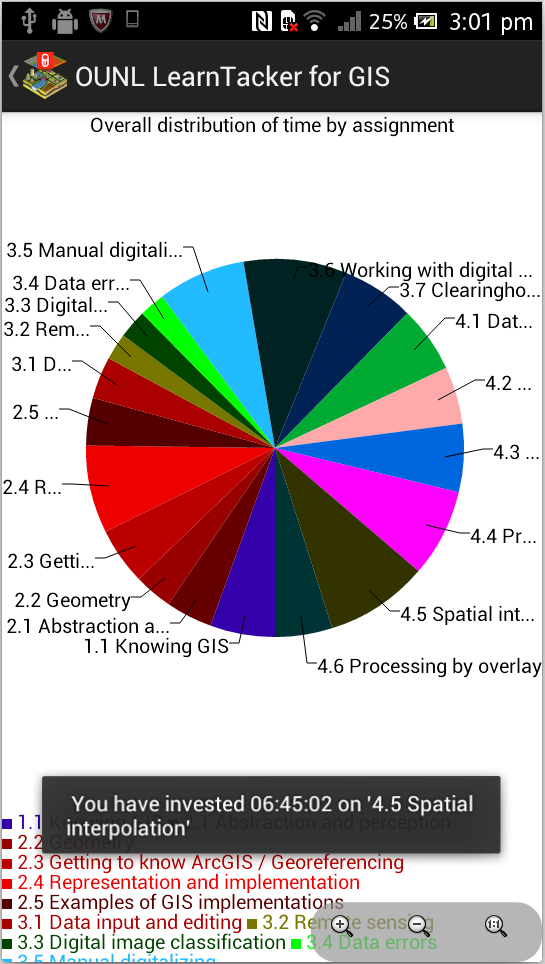
\includegraphics[width=0.3\linewidth]{img/studyload_fig4a}
		\label{fig:sload_4a}
	}
	\subfloat[Linechart. X-axis illus- trates activities in a course. Y-axis represents the number of hours devoted to study. My time (violet line) vs. My colleagues� time (black line)]{
		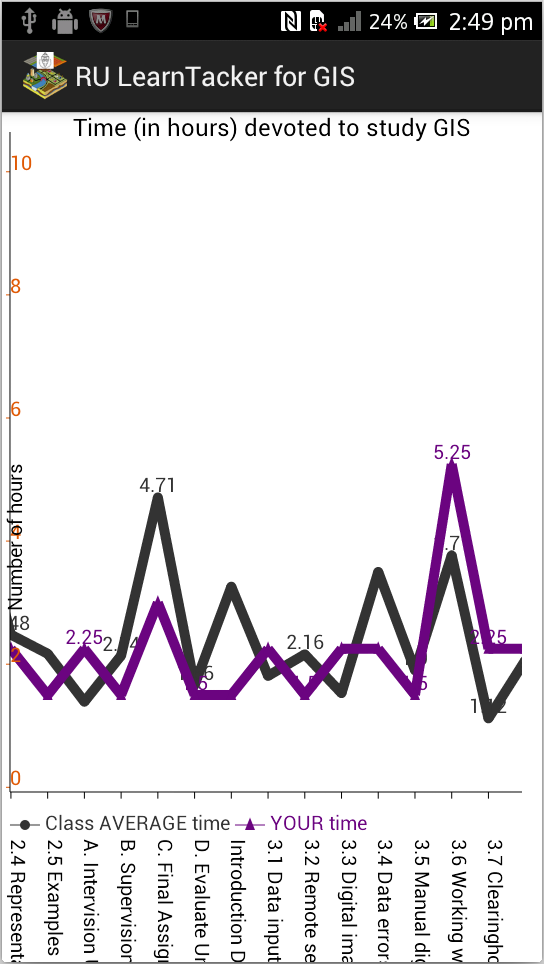
\includegraphics[width=0.3\linewidth]{img/studyload_fig4b}
		\label{fig:sload_4b}
	}	
	\subfloat[Linechart. X-axis illus- trates activities in a course. Y-axis represents number of hours devoted to study. My time (violet line) vs. My colleagues� time (red line) vs. My teacher� estimation (blue line)]{
		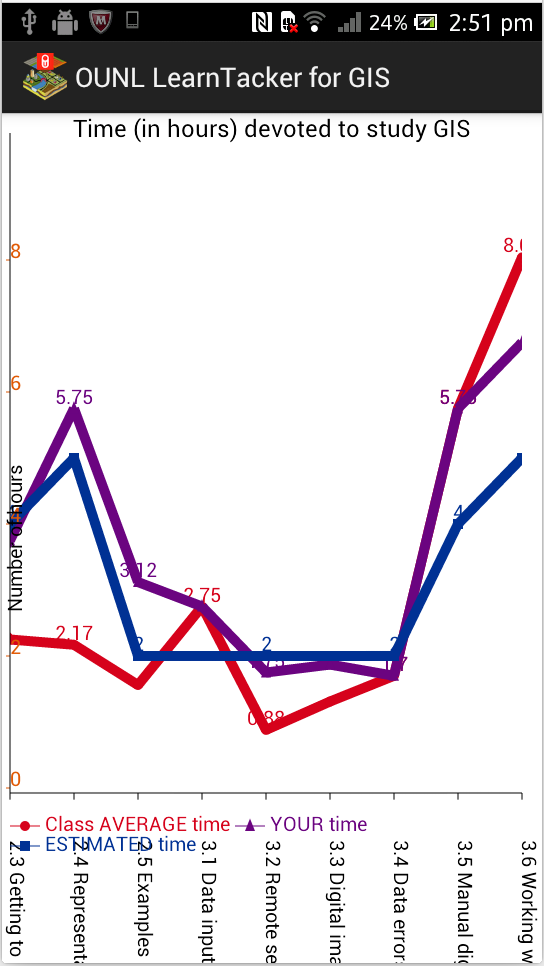
\includegraphics[width=0.3\linewidth]{img/studyload_fig4c}
		\label{fig:sload_4c}
	}	
      \caption{Learning analytics in LearnTracker}
      \label{fig:sload_4}
\end{figure}
\end{center}

\textbf{Multiplatform web interface}



\begin{center}
\begin{figure}[ht]
\centering
	\subfloat[Yardstick]{
		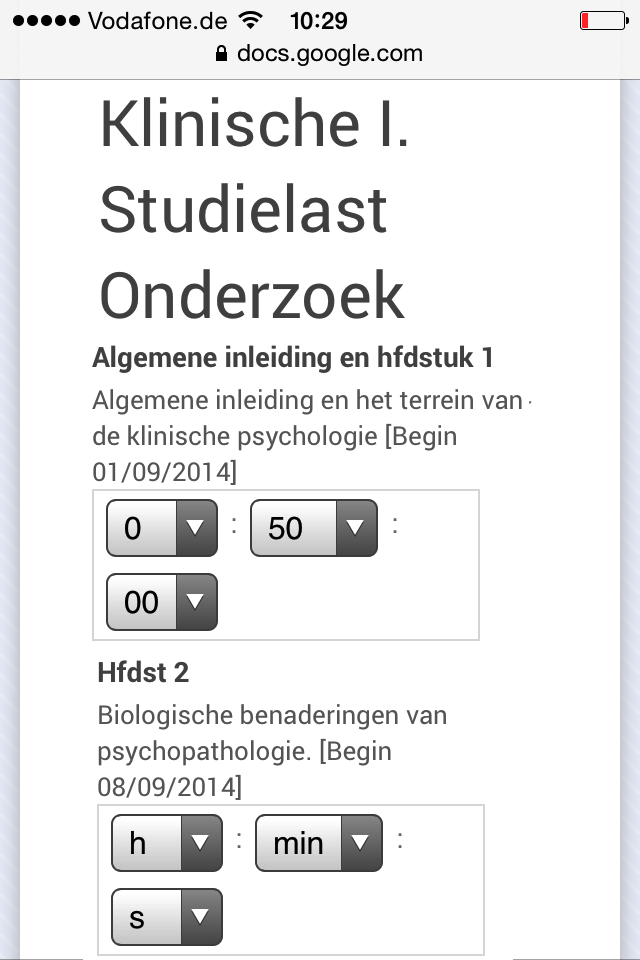
\includegraphics[width=0.3\linewidth]{img/studyload_fig5a}
		\label{fig:sload_5a}
	}
	\subfloat[Piechart. Time devoted to each learning activity]{
		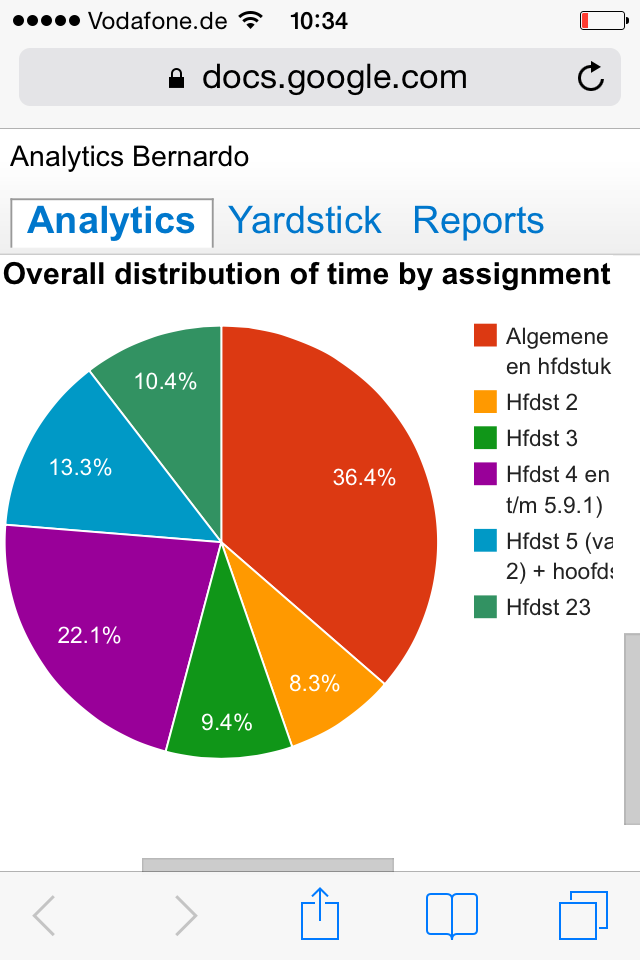
\includegraphics[width=0.3\linewidth]{img/studyload_fig5b}
		\label{fig:sload_5b}
	}	
	\subfloat[Barchart. My time VS time initially scheduled by the teacher]{
		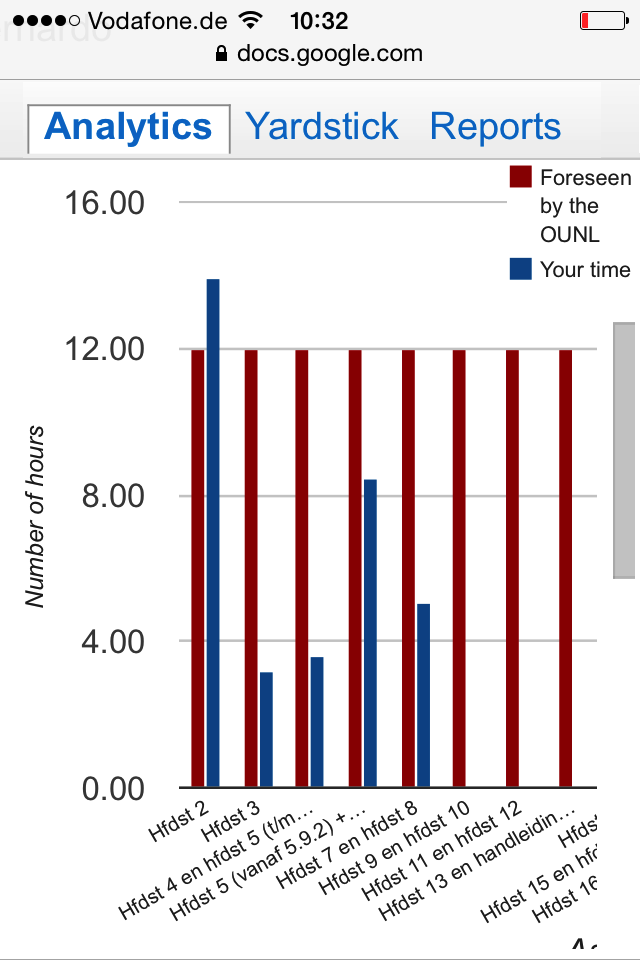
\includegraphics[width=0.3\linewidth]{img/studyload_fig5c}
		\label{fig:sload_5c}
	}	
      \caption{Multiplatform web interface}
      \label{fig:sload_5}
\end{figure}
\end{center}
\subsubsection{Notifications and SMS broadcasting tool}


\begin{center}
\begin{figure}[ht]
\centering
	\subfloat[SMS management tool]{
		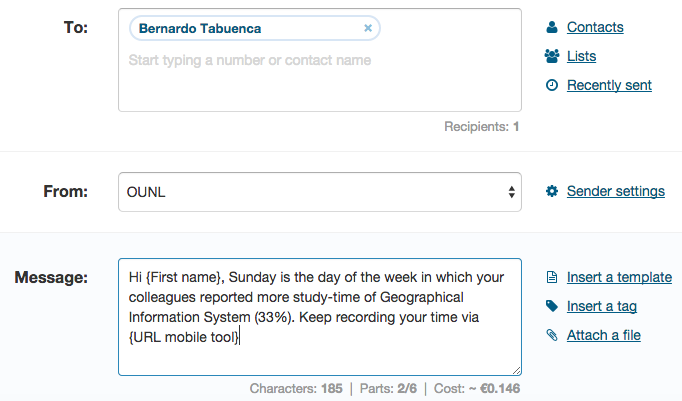
\includegraphics[width=0.3\linewidth]{img/studyload_fig6a}
		\label{fig:sload_6a}
	}
	\subfloat[SMSs generated out of the templates]{
		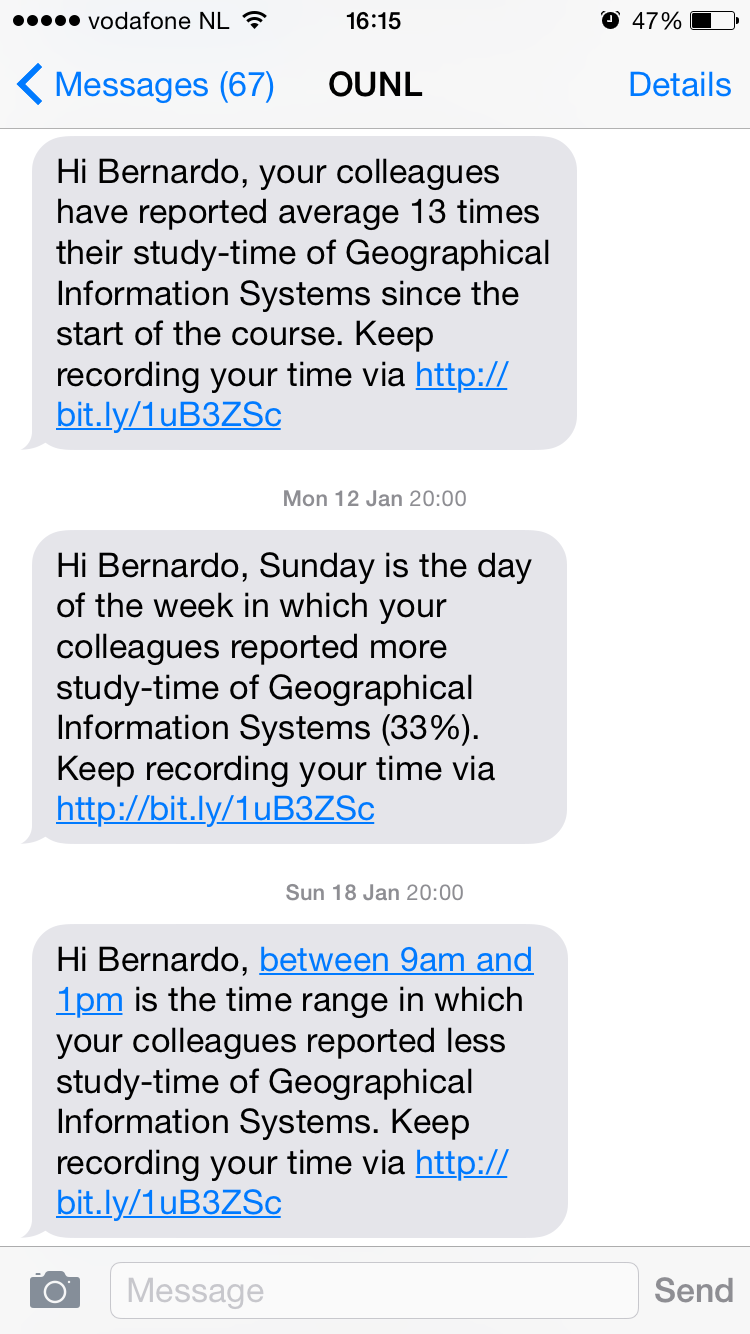
\includegraphics[width=0.3\linewidth]{img/studyload_fig6b}
		\label{fig:sload_6b}
	}		
      \caption{SMS broadcasting tool}
      \label{fig:sload_6}
\end{figure}
\end{center}
\subsection{Design of the experiment}


\begin{figure}
     \centering
     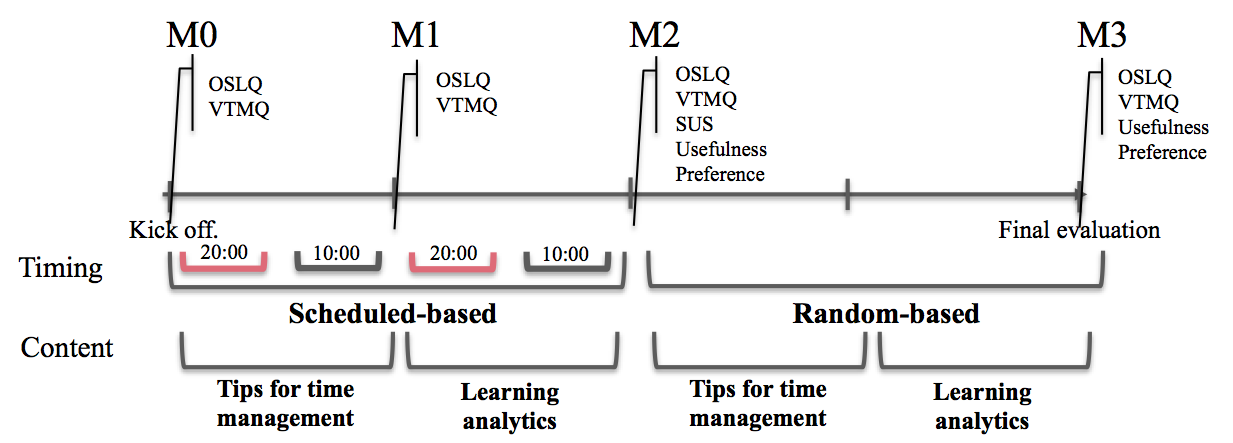
\includegraphics[width=0.7\linewidth]{img/studyload_fig7}
     \caption{Experimental design}
     \label{fig:sload_7}
\end{figure}
\subsection{Measure instruments}

\subsubsection{Self-regulation}

\subsubsection{Validity and reliability of time management}

\subsubsection{Time patterns}

\subsubsection{Complexity of the mobile tool}

\subsection{Procedure}

\subsection{Data analysis}

\section{Results}

\subsection{Impact of logging/monitoring time in self-regulation}

\begin{center}
\begin{figure}[ht]
\centering
	\subfloat[Time management]{
		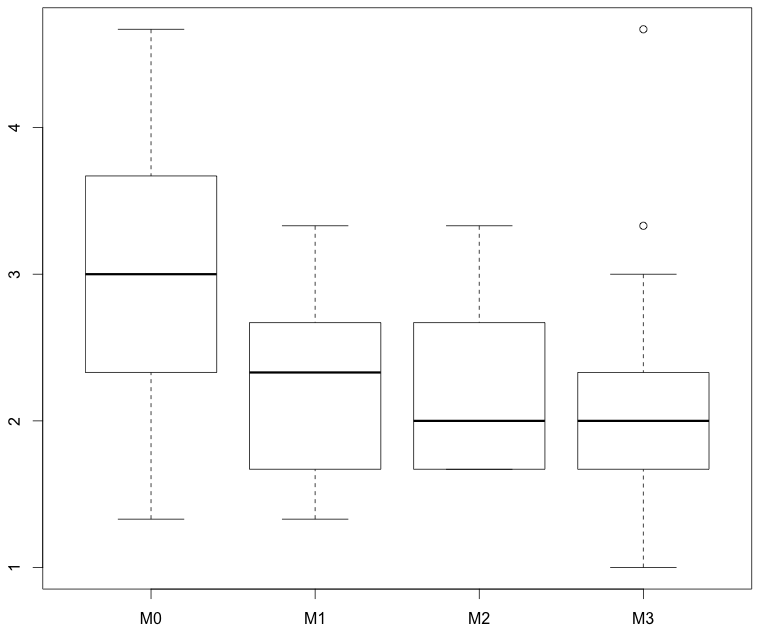
\includegraphics[width=0.3\linewidth]{img/studyload_fig8a}
		\label{fig:sload_8a}
	}
	\subfloat[Time planning]{
		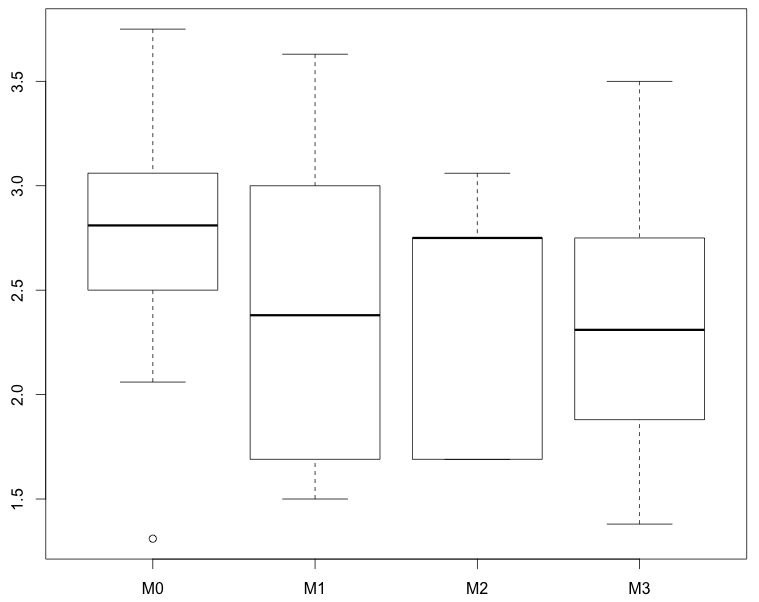
\includegraphics[width=0.3\linewidth]{img/studyload_fig8b}
		\label{fig:sload_8b}
	}	

      \caption{Boxplot with mean scores for significant subscales. 5) Strongly disagree; 4) Disagree; 3) Neutral; 2) Agree; 1) Strongly agree;}
      \label{fig:sload_8}
\end{figure}
\end{center}

\subsection{Impact of the timing in the notifications in self-regulation}

\begin{center}
\begin{figure}[ht]
\centering
	\subfloat[Contrast 1. Notifications pushed at fixed time of the day]{
		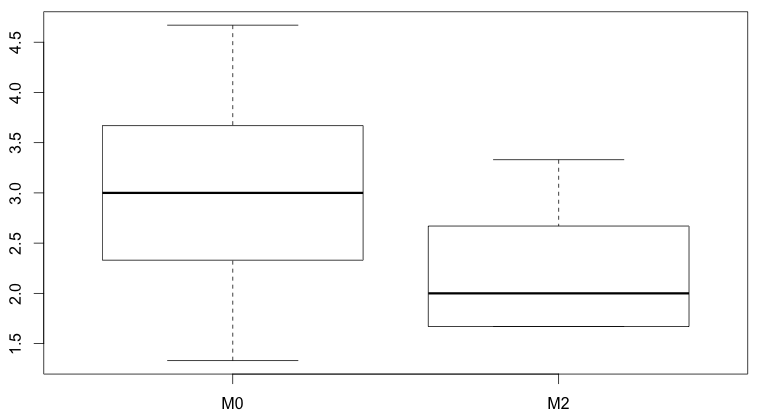
\includegraphics[width=0.3\linewidth]{img/studyload_fig9a}
		\label{fig:sload_9a}
	}
	\subfloat[Contrast 2. Notifications pushed on random basis in the time of the day]{
		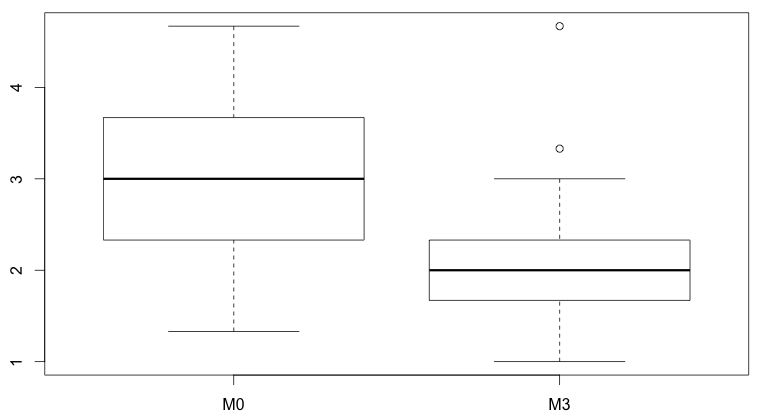
\includegraphics[width=0.3\linewidth]{img/studyload_fig9b}
		\label{fig:sload_9b}
	}	
      \caption{Boxplots with measure of means in �time management� subscale. 5) Strongly disagree; 4) Disagree; 3) Neutral; 2) Agree; 1) Strongly agree;}
      \label{fig:sload_9}
\end{figure}
\end{center}

\subsubsection{Patterns sampling study time}

\begin{figure}
     \centering
     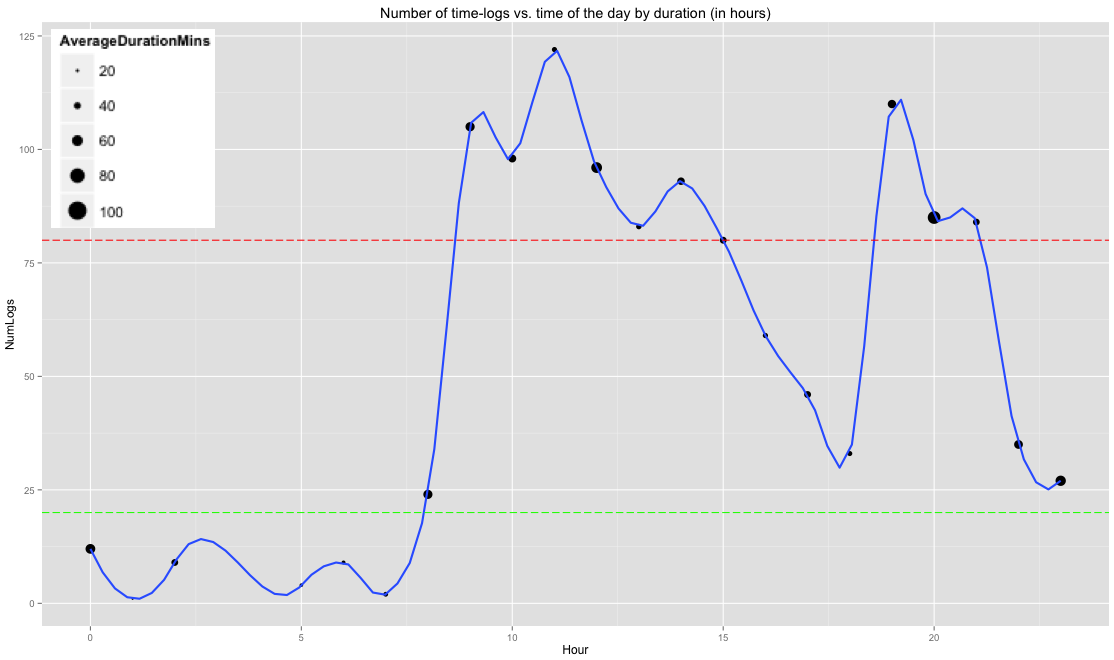
\includegraphics[width=0.7\linewidth]{img/studyload_fig10}
     \caption{Distribution of time logs along the day (n=1217). Y-axis represents the number of time-logs during the day. X-axis represents the time of the day. The width of the plot represents the mean duration of the time-logs for an hour.}
     \label{fig:sload_10}
\end{figure}


\begin{figure}
     \centering
     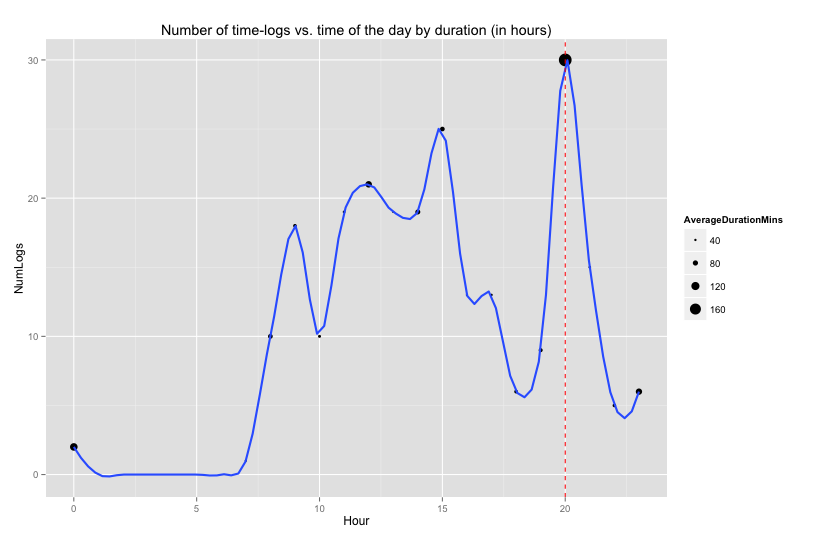
\includegraphics[width=0.7\linewidth]{img/studyload_fig11}
     \caption{Y-axis is the number of logs. X-axis is the time of the day. Relationship between the SMS notifications and students� time-log reactions. Submitting message in the evening at 20h. The thickness of the plot is the duration of the time-logs recorded}
     \label{fig:sload_11}
\end{figure}



\begin{figure}
     \centering
     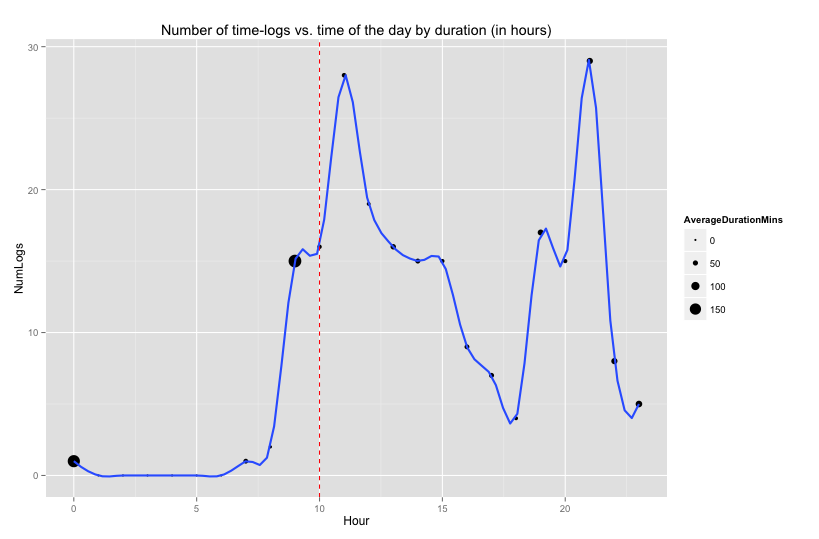
\includegraphics[width=0.7\linewidth]{img/studyload_fig12}
     \caption{Y-axis is the number of logs. X-axis is the time of the day. Relationship between the SMS notifications and students� time-logs reaction. Submitting message in the morning at 10h. The thickness of the plot is the duration of the time-logs recorded.}
     \label{fig:sload_12}
\end{figure}


\begin{figure}
     \centering
     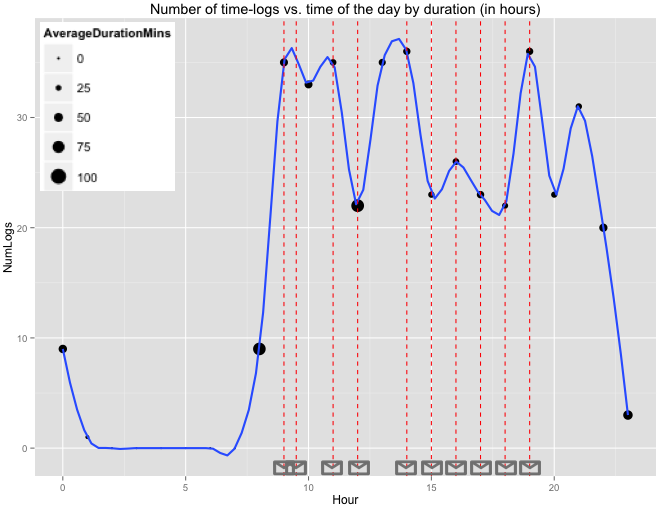
\includegraphics[width=0.7\linewidth]{img/studyload_fig13}
     \caption{Y-axis is the number of logs. X-axis is the time of the day. Relationship between the SMS notifications and students� time-logs reaction. Submitting message on random basis. The thickness of the plot is the duration of the time-logs recorded.}
     \label{fig:sload_13}
\end{figure}


\subsubsection{How do students log their time}

\subsubsection{Correlation between time-logs and performance}


\subsection{Impact from the content of the notifications in self-regulation}


\begin{center}
\begin{figure}[ht]
\centering
	\subfloat[Contrast 1. Notifications containing generic tips]{
		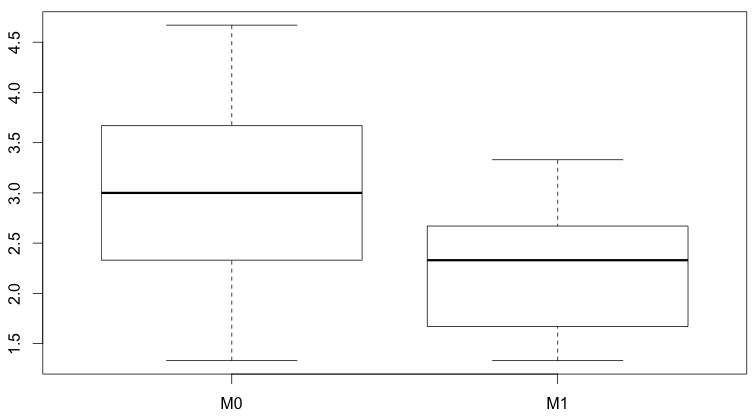
\includegraphics[width=0.3\linewidth]{img/studyload_fig14a}
		\label{fig:sload_14a}
	}
	\subfloat[Contrast 2. Notifications containing learning analytics]{
		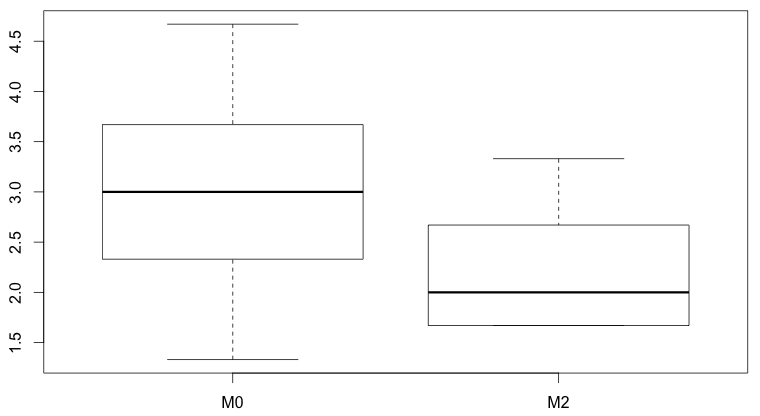
\includegraphics[width=0.3\linewidth]{img/studyload_fig14b}
		\label{fig:sload_14b}
	}		
      \caption{Boxplots with measure of means in �time management� subscale. 5) Strongly disagree; 4) Disagree; 3) Neutral; 2) Agree; 1) Strongly agree;}
      \label{fig:sload_14}
\end{figure}
\end{center}

\subsubsection{Preference in content and channels}


\subsection{Usability of the tool}



\section{Discussion}


\subsection{Interpretation of the results}

\subsection{Limitations}


\subsection{Significance of the study}

